\documentclass[conference]{IEEEtran}

\usepackage{graphicx}
\usepackage{cite,url}
\usepackage{amsmath,amssymb,amsfonts}
\usepackage{textcomp}
\usepackage{xcolor}
\usepackage{amsthm}
\usepackage{booktabs}
\usepackage{array}
\usepackage{tabularx}

\graphicspath{{./}{results/}}

\newtheorem{definition}{Definition}
\newtheorem{proposition}{Proposition}

\DeclareMathOperator*{\argmax}{arg\,max}
\DeclareMathOperator*{\argmin}{arg\,min}
\newcommand{\TV}{\mathrm{TV}}
\newcolumntype{Y}{>{\raggedright\arraybackslash}X}

\def\BibTeX{{\rm B\kern-.05em{\sc i\kern-.025em b}\kern-.08em
T\kern-.1667em\lower.7ex\hbox{E}\kern-.125emX}}

\begin{document}

\title{PrivSAF: An Auditable Database Operator for Channel-Aware Scalar LDP Stuck-at Cleaning}

\author{
\IEEEauthorblockN{Lv Ding, Zhirong Yue, Ghaoui El Othmane, Dan Yu, Yue Fu, Yongle Chen}
\IEEEauthorblockA{Shanxi Key Laboratory of Industrial Internet Security, Taiyuan University of Technology, China\\
Emails: \{dinglv0099, 2024002578, 2023700034\}@link.tyut.edu.cn, \{yudan, fuyue, chenyongle\}@tyut.edu.cn}
}

\maketitle

\begin{abstract}
Private telemetry databases must clean scalar stuck-at and flatline faults after each client has already randomized the raw reading under local differential privacy (LDP). This paper frames the task as a database-operator problem: the server must join privatized reports with the declared channel, select an eligible cleaning operator, maintain privacy and provenance ledgers, replay corrections, and expose repair-aware SQL views without seeing raw values. PrivSAF implements this operator contract for repeated-value scalar faults. Its statistical kernel constrains normal emissions to \(M\alpha\) and stuck emissions to a single declared-channel column \(M_{:,s}\); standard mixture and HMM post-processing then produce posterior cleaning records, stuck-bucket estimates, fault ratios, and posterior masks. The router is a deterministic policy over label semantics, channel separation, validation lift, and cost, so weak or mismatched rows are logged as abstain/route decisions rather than silently treated as detections. On five-stream segment faults, PrivSAF-HMM reaches \(0.930/0.833\) AUROC/AUPRC; on median and minimum-TV \(\varepsilon=2\) stress rows, AUPRC remains \(0.085\) and \(0.079\), near prevalence \(0.075\), which motivates the validation-lift gate. Real-label evidence is boundary-tiered: HadISD straight-string flags support repeated-value semantics, NOAA CO-OPS provides only weak private flat-tolerance lift (\(0.539/0.0246\) AUROC/AUPRC), and I-ORS/WSN labels are routed to local-regime statistics. The prototype implements the operator contract with immutable privatized-report storage, versioned policy and calibration metadata, replayable posterior records, provenance links, and repair-aware aggregate views.
\end{abstract}

\section{Introduction}
\label{sec:introduction}

Scalar telemetry warehouses increasingly collect reports through client-side local differential privacy (LDP). When a sensor becomes stuck before randomization, the database receives only privatized samples whose exact values need not repeat. A cleaning stage therefore cannot run ordinary flatline rules over raw readings. It must reason over the declared randomization channel, preserve the per-report privacy boundary, record why a derived cleaning decision was made, and let downstream SQL analyses compare unrepaired and posterior-mask repaired aggregates.

We treat this as a data-management problem rather than only a scoring problem. The input relation contains immutable privatized reports, mechanism identifiers, privacy budgets, and calibration versions. Beyond scoring, the operator must make each posterior decision replayable and auditable under a declared LDP channel. It therefore joins reports with a public channel matrix, selects an operator compatible with the semantic layer, emits versioned posterior records instead of overwriting facts, and preserves the metadata needed to explain late corrections. A script can compute a stuck-at score, but it does not by itself define these replay, provenance, and repair-aware query semantics.

PrivSAF is the resulting auditable operator for scalar repeated-value faults. The statistical step is intentionally compact: normal readings emit \(b_0=M\alpha\), while a raw stuck bucket \(s\) emits \(b_1=M_{:,s}\). An iid mixture handles point stuck-at faults, a two-state HMM handles persistent flatlines, and a dropout HMM handles explicit availability symbols. The database-facing contribution is the binding between these channel-constrained emissions and an operator contract that exposes posterior fault scores, stuck-bucket estimates, fault ratios, posterior-mask repair aids, and lineage from each output back to the privatized reports and policy version that produced it.

The scope is deliberately precise. Central or minimum-TV stuck values, low \(\varepsilon\), contaminated calibration, short traces, and labels that encode local quality-control regimes can make stuck-column inference weak. PrivSAF therefore includes a router that first checks semantic compatibility, then records TV/KL separation, then requires validation lift before deployment. HadISD straight-string labels match repeated-value semantics; NOAA CO-OPS flat-tolerance labels provide weak official value+label evidence; I-ORS and WSN labels behave more like local-regime or row-preparation labels and are routed to GLR/CUSUM-style statistics.

The database evidence is evaluated alongside detection utility. The artifact implements the same contract across SQLite, DuckDB, and PostgreSQL paths, including batch likelihood materialization, temporal posterior state, replay/correction lineage, and repair-aware aggregate queries. This framing addresses the central deployment question: not only whether a known-channel score works, but whether private stuck-at cleaning can be replayed, audited, and queried as a first-class database operator.

The pipeline is deliberately split at the privacy boundary: client devices produce PM-LDP reports, while the server only post-processes privatized report buckets and public or separately accounted metadata. PrivSAF builds normal, stuck-at, and dropout emissions, then emits posterior fault scores, stuck-bucket summaries, posterior masks, and provenance records. The router chooses among PrivSAF, GLR, LLR-CUSUM, dropout HMM, and PM-window operators when scalar labels share similar names but differ in persistence, availability, or local-regime semantics.

The contributions are as follows:
\begin{itemize}
    \item \textbf{A database operator contract for private cleaning.} PrivSAF defines an auditable contract for privatized report storage, declared-channel lookup, policy/calibration metadata, posterior state, privacy/provenance accounting, replay, and repair-aware SQL aggregates for scalar LDP cleaning.
    \item \textbf{Channel-constrained emissions for scalar stuck-at inference.} The operator maps a declared scalar LDP channel into normal emission \(M\alpha\) and stuck emission \(M_{:,s}\). Mixture/HMM inference remains standard post-processing, but the emission family is tied to raw stuck-at semantics and to derived database records.
    \item \textbf{A deterministic audit router.} The routing policy combines semantic compatibility, TV/KL separation, validation lift, and explicit false-accept accounting. TV/KL diagnostics admit a candidate to validation; they do not certify deployment utility by themselves.
    \item \textbf{Boundary-aware evidence and artifact.} The evaluation separates model-matched successes from central/min-TV failures and semantic mismatches, and the artifact demonstrates replayable operator execution, correction lineage, privacy-ledger checks, and posterior-mask aggregate views.
\end{itemize}


\section{Problem Statement}
\label{sec:problem}

\subsection{Private Stream Model}
Consider a sensing stream represented as a time-indexed sequence
\[
\mathbf{v}=\{v_1,\ldots,v_n\},
\]
where \(v_t\in[-1,1]\) after normalization. At each time \(t\), the client applies an \(\varepsilon\)-LDP mechanism \(\mathcal{M}\) and uploads only
\[
x_t=\mathcal{M}(v_t).
\]
The server observes the privatized stream
\[
\mathbf{x}=\{x_1,\ldots,x_n\},
\]
but not the raw stream \(\mathbf{v}\).

The server-side cleaning goal is to:
\begin{enumerate}
    \item choose a scalar stuck-at/flatline cleaning operator from the declared channel, label semantics, and validation evidence;
    \item detect intermittent stuck-at or flatline faults using per-time posterior scores when the stuck-at model matches the label;
    \item estimate the fault ratio and stuck-at bucket when applicable;
    \item route explicit availability labels and local quality-control changes to the matching scalar channel statistic;
    \item optionally produce a posterior-mask repair aid or smoothed sequence estimate and provenance record for downstream analytics.
\end{enumerate}

All outputs are diagnostics computed from \(\mathbf{x}\), public mechanism parameters, scalar-domain metadata, and calibration hyperparameters; raw readings \(\mathbf{v}\) and labels \(\mathbf{z}\) are unavailable to the server. The same channel interface also supports PM-window GLR and LLR-CUSUM for local quality-control regime changes, and a dropout HMM when an explicit availability symbol is present. PrivSAF remains the posterior operator for true stuck-at/flatline semantics.

\noindent\emph{Auditable deployment policy.}
Let \(\mathcal{O}=\{\textsc{Mix},\textsc{HMM},\textsc{Scan},\textsc{GLR},\textsc{CUSUM},\textsc{Drop}\}\) denote the candidate scalar operators, and let \(g\) be a label stratum such as iid stuck, persistent flatline, deployed QC stuck, or explicit availability. The policy first restricts candidates through a semantic compatibility set
\[
\mathcal{C}(g)\subseteq\mathcal{O}.
\]
For example, \(\mathcal{C}(\text{persistent flatline})=\{\textsc{HMM},\textsc{Scan}\}\), \(\mathcal{C}(\text{iid stuck})=\{\textsc{Mix}\}\), \(\mathcal{C}(\text{deployed QC stuck})=\{\textsc{GLR},\textsc{CUSUM},\textsc{HMM}\}\), and \(\mathcal{C}(\text{availability})=\{\textsc{Drop}\}\). Given validation rows \(V_g\), empirical utility \(\widehat U_o(V_g)\) (AUPRC in the experiments), and per-frame cost \(c_o\), the selected operator is
\[
o^\star(g)=
\arg\max_{o\in\mathcal{C}(g)}
\left\{\widehat U_o(V_g)-\lambda c_o\right\}.
\]
For stuck-column candidates, the policy also records separation
\[
\TV(M_{:,s},M\alpha)
\quad\text{and}\quad
D_{\mathrm{KL}}(M_{:,s}\|M\alpha).
\]
The separation audit uses fixed thresholds \(\TV\ge0.10\) and \(D_{\mathrm{KL}}\ge0.03\). Rows below either threshold are marked to abstain or route; compatible GLR/CUSUM/window operators can still be selected by validation. Rows above both thresholds only enter validation-utility selection. To make the lift requirement explicit, let \(\pi_g\) be the validation prevalence for semantic layer \(g\), and define
\[
L_o(g)=\frac{\widehat U_o(V_g)}{\max(\pi_g,10^{-6})}.
\]
A stuck-column deployment requires both separation and \(L_o(g)\ge\tau_{\mathrm{lift}}\); otherwise the operator emits audit records or routes to the best compatible alternative. We set \(\tau_{\mathrm{lift}}=2\) for all deployment-facing router decisions, matching the \(2\times\) prevalence threshold used in the false-accept audit. The experiments set \(\lambda=0\) for accuracy tables and report runtime separately.

This policy is deterministic once \(\mathcal{C}(g)\), the separation thresholds, \(\tau_{\mathrm{lift}}\), validation rows, and cost weight are fixed. Compatible operators are restricted before validation scoring, validation AUPRC selects among those operators, and held-out test rows are used only for final reporting. Boundary cases are therefore represented as routing outcomes: I-ORS and WSN are semantic-mismatch layers where local QC/regime statistics outperform the global stuck-column posterior.

The deployment order is semantic compatibility \(\rightarrow\) TV/KL audit \(\rightarrow\) validation lift \(\rightarrow\) final operator selection, abstention, or route. The artifact materializes this order as ledgers with columns for semantic layer, dataset, privacy budget, stuck-value type, TV/KL separation, selected action, selected method, validation AUPRC/lift, diagnostic stage, candidate-bucket source, test AUPRC for final reporting, and evidence file. The candidate-bucket source field uses a fixed vocabulary: synthetic audit bucket, selected candidate, top-\(k\) candidate, or validation-selected candidate. In synthetic audit rows, the true stuck bucket is used only to audit the benchmark; operational deployments must use selected, top-\(k\), or validation-selected candidates. Test labels are never used in routing.

\noindent\emph{Label-efficient deployment.}
Validation labels and router evidence are public benchmark evidence in this paper. If operational labels are sensitive, they require separate privacy accounting or access control. If labels are absent or too sparse to estimate validation lift, PrivSAF runs in audit/triage mode: it can emit candidate posteriors, separation diagnostics, and provenance, but it should remain in audit/triage mode before auto-repairing production aggregates.

\subsection{Local Differential Privacy and Post-Processing}

\begin{definition}[Local Differential Privacy \cite{kasiviswanathan2011what}]
A randomized mechanism \(\mathcal{M}\) satisfies \(\varepsilon\)-LDP if for any \(u,u'\in[-1,1]\) and any measurable set \(\mathcal{S}\),
\[
\Pr[\mathcal{M}(u)\in\mathcal{S}]
\le
e^{\varepsilon}
\Pr[\mathcal{M}(u')\in\mathcal{S}].
\]
\end{definition}

\begin{proposition}[Post-processing \cite{dworkroth2014}]
Any data-independent algorithm applied only to privatized reports does not weaken the LDP guarantee of \(\mathcal{M}\).
\end{proposition}

\begin{proposition}[PrivSAF pipeline privacy]
Fix a public mechanism table, clipping bounds, calibration version, router policy, and query workload. If every client report is generated by an \(\varepsilon_t\)-LDP scalar mechanism, then the complete server-side PrivSAF pipeline---operator selection, candidate search, posterior scoring, event-window construction, posterior-mask repair-aid generation, provenance rows, materialized views, and SQL analytics over those derived tables---is \(\varepsilon_t\)-LDP for each reported scalar value. For a trajectory from one device, basic sequential composition gives privacy cost \(\sum_t \varepsilon_t\) for the selected privacy unit.
\end{proposition}

\begin{proof}[Proof sketch]
All listed outputs are deterministic or randomized functions of the privatized report ledger and public metadata. They do not query the raw scalar values. The post-processing theorem preserves the per-report LDP guarantee, and sequential composition gives the trajectory-level statement.
\end{proof}

\noindent\emph{Privacy scope and deployment ledger.}
PrivSAF inherits the data-collection guarantee. Each client clips/normalizes with public, client-side, or separately accounted constants and applies PM with per-report budget \(\varepsilon_t\), giving pure \(\varepsilon_t\)-LDP for one scalar report. The paper reports per-report budgets; a device trajectory has basic-composition cost \(\sum_t\varepsilon_t\), so long-running deployments need report caps or a longitudinal accountant. The artifact includes a device-level ledger; at a 10-minute cadence, \(\varepsilon=0.5\) consumes \(72\) privacy units/day, so budget \(10\) covers 20 reports. If availability itself is sensitive, dropout must be sent through cover traffic or a separately accounted LDP bit.

Thus the accounting boundary is simple: client scalar randomization consumes the per-report \(\varepsilon_t\); posterior scoring, candidate search, routing, repair aids, provenance, and SQL analytics are post-processing. Clipping, calibration, validation labels, or availability signals that are learned from sensitive data require their own accounting or access control.

\subsection{Piecewise Mechanism for Real-Valued Reports}
\label{sec:pm}

We instantiate \(\mathcal{M}\) using the Piecewise Mechanism (PM), a standard mechanism for real-valued LDP analytics \cite{wang2019multidimensional}. For privacy budget \(\varepsilon\), define
\[
C =
\frac{e^{\varepsilon/2}+1}{e^{\varepsilon/2}-1}.
\]
For input \(v\in[-1,1]\), PM defines the high-density interval
\[
\ell(v)=\frac{e^{\varepsilon/2}v-1}{e^{\varepsilon/2}-1},
\qquad
r(v)=\frac{e^{\varepsilon/2}v+1}{e^{\varepsilon/2}-1}.
\]
The output \(x\in[-C,C]\) is sampled from the piecewise density
\begin{equation}
f(x\mid v)=
\begin{cases}
\frac{e^{\varepsilon/2}}{e^{\varepsilon/2}+1}\cdot \frac{1}{C-1},
& x\in[\ell(v),r(v)],\\[4pt]
\frac{1}{e^{\varepsilon/2}+1}\cdot \frac{1}{C+1},
& \text{otherwise}.
\end{cases}
\label{eq:pm-pdf}
\end{equation}

\subsection{Intermittent Stuck-at Faults}
\label{sec:faultmodel}

A stuck-at fault occurs before privatization: the raw sensing channel becomes fixed at a constant value for a set of time indices.

\begin{definition}[Intermittent stuck-at fault]
A stream exhibits intermittent stuck-at faults if there exists a set \(A\subseteq\{1,\ldots,n\}\) and a constant \(a\in[-1,1]\) such that \(v_t=a\) for all \(t\in A\). The frame-level label is \(z_t=\mathbb{I}[t\in A]\).
\end{definition}

Under LDP, the server observes a randomized report \(x_t\) rather than the raw value \(v_t\). PrivSAF therefore performs probabilistic inference and outputs
\[
\gamma_t=\Pr[z_t=1\mid \mathbf{x}],
\]
which is used as the anomaly score.

\section{PrivSAF}
\label{sec:method}

\subsection{Channel Model and Calibration}
\label{sec:method_overview}

PrivSAF is a targeted server-side post-processing method for locally private scalar streams. The client first normalizes or bounds the raw value and applies an LDP mechanism. The server then uses the known channel matrix to infer latent stuck-at structure. PrivSAF supports two closely related models:
\begin{itemize}
    \item an independent mixture model, which is useful for controlled parameter estimation and ablation;
    \item a persistent segment scorer, implemented with a standard two-state HMM backend, for segment-level intermittent faults.
\end{itemize}
Both variants estimate the normal distribution, stuck-at bucket, fault ratio, and posterior fault scores.

The segment backend is compact; the distinctive step is emission construction. Each privatized-report probability is obtained by marginalizing the known channel over normal and stuck-at raw buckets. The HMM machinery is standard, but its emissions are constrained by the LDP channel and raw stuck-at semantics, enabling stuck-bucket estimation, channel-miscalibration tests, and posterior-mask repair aids under post-processing.

\noindent\emph{Discretization and PM transition matrix.}
\label{sec:discretization}

We discretize the raw domain \([-1,1]\) into \(d\) buckets \(\{B_i\}_{i=1}^{d}\) with centers \(c_i\), and discretize the PM output domain \([-C,C]\) into \(\tilde d\) buckets \(\{\tilde B_j\}_{j=1}^{\tilde d}\). Each privatized report \(x_t\) is mapped to an output bucket \(j(t)\).

The PM channel is represented by a transition matrix
\[
M\in\mathbb{R}^{\tilde d\times d},
\qquad
M_{j,i}=\Pr[x\in\tilde B_j\mid v=c_i].
\]
Let \(I_i=[\ell(c_i),r(c_i)]\). Using the PM densities in Eq.~\eqref{eq:pm-pdf}, define
\[
f_{\mathrm{in}}=
\frac{e^{\varepsilon/2}}{e^{\varepsilon/2}+1}\cdot \frac{1}{C-1},
\qquad
f_{\mathrm{out}}=
\frac{1}{e^{\varepsilon/2}+1}\cdot \frac{1}{C+1}.
\]
Then each matrix entry is computed exactly by interval integration:
\begin{equation}
M_{j,i}
=
f_{\mathrm{in}}\cdot |\tilde B_j\cap I_i|
+
f_{\mathrm{out}}\cdot |\tilde B_j\setminus I_i|,
\label{eq:transition}
\end{equation}
where \(|\cdot|\) denotes interval length. This construction makes the server-side inference numerically stable and explicitly tied to the LDP mechanism.

\noindent\emph{Mechanism-general channel interface.}
PrivSAF only requires a column-stochastic matrix \(M\), where \(M_{j,i}\) is the probability that raw bucket \(i\) emits report symbol or bucket \(j\). PM is the main channel, but any discretized real-valued LDP mechanism can be substituted. The mechanism extension uses the Duchi binary mechanism, whose \(+1\) report probability for raw bucket center \(c_i\) is
\[
\Pr[y=+1\mid c_i]
=
\frac{1}{2}
+
\frac{c_i}{2}\cdot\frac{e^\varepsilon-1}{e^\varepsilon+1},
\]
and the \(-1\) probability fills the other row of a \(2\times d\) channel matrix. No inference step changes after this substitution; only \(M\) and the report alphabet change. The mechanism panel then reports utility separately for each channel and privacy budget.

\noindent\emph{Calibration and initialization.}
\label{sec:calibration}

PrivSAF assumes that the scalar domain, bucketization, LDP mechanism parameters, and clipping/normalization constants are fixed before server-side inference. These constants must be public, configured on the client, obtained from non-sensitive calibration data, or learned with a separately accounted privacy mechanism. The server-side inference in PrivSAF does not require raw operational readings.

The normal emission \(b_0=M\boldsymbol{\alpha}\) can be initialized from public calibration, same-mechanism privatized commissioning reports, or a uniform prior. Private calibration reports consume their own budget and enter the longitudinal ledger. In the benchmarks, training splits set preprocessing and calibration before validation/test faults are injected; held-out raw values are used only by the simulator for fault injection and metrics.

Runs initialized from an unprivatized clean raw histogram are labeled as oracle-initialization ablations and excluded from the main private claims. Mild calibration contamination is handled through subsequent EM or Baum--Welch re-estimation; if contamination makes \(M\boldsymbol{\alpha}\) indistinguishable from a stuck-at column, the separation diagnostics in Sec.~\ref{sec:theory} expose that failure mode.

\subsection{Inference Models}
\label{sec:mixture}

\noindent\emph{Independent mixture model under LDP.}
The independent mixture model assumes that each raw bucket is generated by either a normal component or a stuck-at component:
\begin{itemize}
    \item Normal state: \(v_t\in B_i\) with probability \(\alpha_i\), where \(\boldsymbol{\alpha}=(\alpha_1,\ldots,\alpha_d)\) and \(\sum_i\alpha_i=1\).
    \item Fault state: \(v_t\) belongs to a single unknown bucket \(B_{t^\star}\).
\end{itemize}
Let \(r=\Pr[z_t=1]\) be the fault ratio. For output bucket \(j\), the likelihood is
\begin{equation}
\Pr[j(t)=j]
=
(1-r)\sum_{i=1}^{d}\alpha_iM_{j,i}
+
rM_{j,t^\star}.
\label{eq:mix}
\end{equation}

Given candidate \(t^\star\), the E-step computes the posterior fault probability
\begin{equation}
\begin{aligned}
\gamma_t
&=
\Pr[z_t=1\mid j(t)] \\
&=
\frac{rM_{j(t),t^\star}}
{(1-r)\sum_{i=1}^{d}\alpha_iM_{j(t),i}+rM_{j(t),t^\star}}.
\end{aligned}
\label{eq:gamma}
\end{equation}
It also computes the posterior distribution over normal buckets:
\begin{equation}
p_{t,i}
=
\Pr[v_t\in B_i\mid z_t=0,j(t)]
=
\frac{\alpha_iM_{j(t),i}}
{\sum_{k=1}^{d}\alpha_kM_{j(t),k}}.
\label{eq:pti}
\end{equation}
The M-step updates
\begin{equation}
r
\leftarrow
\frac{1}{n}\sum_{t=1}^{n}\gamma_t,
\qquad
\alpha_i
\leftarrow
\frac{\sum_{t=1}^{n}(1-\gamma_t)p_{t,i}}
{\sum_{t=1}^{n}(1-\gamma_t)}.
\label{eq:mstep}
\end{equation}
The stuck-at bucket \(t^\star\) is selected by discrete likelihood search. The EM procedure follows the standard monotonic-likelihood principle \cite{dempster1977em}.

\noindent\emph{Persistent segment scorer.}
\label{sec:hmm}

Intermittent faults are often segment-level rather than isolated point anomalies. Therefore, PrivSAF uses a persistent segment scorer for flatline-style faults. The scorer is implemented as a standard two-state HMM backend whose hidden state \(z_t\in\{0,1\}\) denotes normal or faulty. The transition parameters are
\[
\begin{aligned}
\pi_1&=\Pr[z_1=1],\\
p_{01}&=\Pr[z_t=1\mid z_{t-1}=0],\\
p_{11}&=\Pr[z_t=1\mid z_{t-1}=1].
\end{aligned}
\]
The normal emission probability in the privatized domain is
\begin{equation}
b_0(j;\boldsymbol{\alpha})
=
\sum_{i=1}^{d}\alpha_iM_{j,i},
\label{eq:hmm-normal-emission}
\end{equation}
and the stuck-at emission probability is
\begin{equation}
b_1(j;t^\star)=M_{j,t^\star}.
\label{eq:hmm-fault-emission}
\end{equation}

For each candidate \(t^\star\), the segment backend runs Baum--Welch inference on the LDP observation sequence. The model jointly estimates
\[
\hat{\boldsymbol{\alpha}},
\quad
\hat r,
\quad
\hat t^\star,
\quad
\hat\pi_1,
\quad
\hat p_{01},
\quad
\hat p_{11},
\quad
\{\hat\gamma_t\}_{t=1}^{n}.
\]
Here \(\hat\gamma_t\) is the posterior probability that frame \(t\) belongs to the stuck-at state, \(\hat r\) is the estimated overall fault ratio, \(\hat t^\star\) is the estimated stuck-at bucket, and \(\hat{\boldsymbol{\alpha}}\) is the estimated normal distribution.

Operationally, the backend enumerates candidate stuck buckets at \(d=\tilde d=32\), initializes \(\boldsymbol{\alpha}\) from calibration or a uniform prior, runs forward--backward and Baum--Welch updates for each candidate, and returns the highest-likelihood stuck bucket with its posterior stream. The artifact also includes a top-\(k\) online variant for lower-latency streams.

\noindent\emph{Dropout emission extension.}
\label{sec:dropout_model}

The same channel-aware formulation extends to faults whose symptom is availability rather than a fixed raw value. For dropout, the observation alphabet is augmented with a missing symbol \(\bot\). If \(r(j)=\sum_i\alpha_iM_{j,i}\) is the normal predictive PM distribution, the two-state dropout HMM uses
\[
\begin{aligned}
\Pr[x_t=\bot\mid z_t=0]&=\rho_N,\\
\Pr[x_t=j\mid z_t=0]&=(1-\rho_N)r(j),
\end{aligned}
\]
and
\[
\begin{aligned}
\Pr[x_t=\bot\mid z_t=1]&=\rho_D,\\
\Pr[x_t=j\mid z_t=1]&=(1-\rho_D)r(j),
\end{aligned}
\]
with \(\rho_D>\rho_N\). The posterior \( \Pr[z_t=1\mid \mathbf{x}]\) is computed by the same forward--backward machinery used for stuck-at segments. This extension tests availability faults under the same emission-channel view. It assumes that \(\bot\) is an observed report symbol under the same contribution ledger; if the act of not sending a value is sensitive, clients must use cover traffic or privatize the availability bit, and that additional mechanism must be accounted separately.

\subsection{Separation Diagnostics and Routing Assumptions}
\label{sec:theory}

This subsection keeps the diagnostics needed for the router: repeated privatized values fail under continuous PM-LDP, known-channel likelihood is informative when \(q_s\ne r\), and larger privacy budgets improve raw-column separation. These statements justify a separation audit diagnostic, not deployment readiness. 

The HMM rows rely on the usual finite-sample and identifiability conditions for a two-state known-emission model. The declared PM columns should be distinct enough that \(b_0=M\alpha\) differs from the candidate stuck emission \(b_1=M_{:,s}\); the temporal process should be persistent enough that \(p_{11}>p_{01}\); the emission family used in the fit should have restricted rank rather than arbitrary free fault emissions; and calibration should be consistent with the deployment stream or explicitly versioned as a sensitivity condition. When these assumptions fail, the TV/KL diagnostic and validation-lift policy should abstain or route rather than certify utility.

\begin{proposition}[Known-channel likelihood diagnostic statement]
\label{prop:channel-advantage}
For a candidate window of length \(m\), let the normal privatized distribution be
\[
r(j)=\sum_i p(i)M_{j,i},
\]
and let the stuck-at distribution for raw bucket \(s\) be \(q_s(j)=M_{j,s}\). If \(q_s=r\), no test using only privatized observations can distinguish the two hypotheses. If \(q_s\ne r\), the statistic
\[
\Lambda_m=\sum_{t=1}^{m}\log\frac{q_s(j(t))}{r(j(t))}
\]
is the Neyman--Pearson optimal test and has positive per-sample separation \(D(q_s\|r)\) under the fault. Under continuous PM outputs, for any \(m\ge2\),
\[
\Pr[x_1=x_2=\cdots=x_m\mid v_1=\cdots=v_m=s]=0,
\]
so exact flatline tests applied to PM reports have zero power. For discretized PM outputs, if a bucket-count test declares faults only when observations in an output bucket \(B_s\) are unusually frequent and \(q_s(B_s)\le r(B_s)\), then its true-positive rate is no larger than its false-positive rate at every such threshold.
\end{proposition}

\begin{proposition}[PM emission-separation diagnostic statement]
\label{prop:pm-separation}
Let \(P_v^\varepsilon\) be the continuous PM output law for input \(v\in[-1,1]\), and let \(s=e^{\varepsilon/2}\). For any \(u,v\in[-1,1]\),
\[
\TV(P_v^\varepsilon,P_u^\varepsilon)
=
\min\left\{
\frac{s-1}{2}|v-u|,
\;
1-\frac{1}{s}
\right\}.
\]
Therefore the PM output laws of two distinct raw values become more separated as \(\varepsilon\) increases. For regular output discretization, the discrete column distance satisfies
\[
\lim_{\tilde d\rightarrow\infty}
\frac{1}{2}\|M_{:,i}-M_{:,k}\|_1
=
\TV(P_{c_i}^\varepsilon,P_{c_k}^\varepsilon).
\]
\end{proposition}

These diagnostic statements give a practical audit signal rather than a deployment guarantee. If \(b_0=M\alpha\) equals or approaches a candidate stuck column \(M_{:,s}\), normal and stuck-at emissions are observationally indistinguishable or weakly distinguishable after privatization; larger \(\varepsilon\) improves PM column separation, but central stuck values can still be hard when \(M\alpha\) places substantial mass near the same output buckets. The experiments use \(\TV(M_{:,s},M\alpha)\) and \(D_{\mathrm{KL}}(M_{:,s}\|M\alpha)\) as necessary but not sufficient diagnostics for whether PrivSAF should be used, abstained, or routed to a compatible local statistic.

\subsection{Implementation and Database Contract}
\label{sec:implementation}

The reported runs use full candidate enumeration at \(d=\tilde d=32\). Larger deployments use three post-processing optimizations. First, iid mixture updates use materialized report-bucket counts, reducing each EM iteration from \(O(nd)\) to \(O(\tilde d d)\). Second, candidate search can shortlist the top \(k\ll d\) stuck columns using a coarse mixture residual before running temporal refinement. Third, the stream implementation maintains keyed filtering probabilities, transition counts, discounted bucket weights, calibration id, and replay id. The measured top-8 online segment backend reduces per-frame time from \(0.374\) ms to \(0.125\) ms, with lower accuracy than full enumeration.

\noindent\emph{Database integration.}
\label{sec:db_integration}

PrivSAF is intended to run as a stateful cleaning operator inside a private telemetry ingestion pipeline. Its input contract is
\[
\texttt{Clean}_{\theta}(R,M,C,P) \rightarrow (D,S,A),
\]
where \(R\) is the immutable \(\texttt{LDP\_REPORTS}\) relation, \(M\) is the declared \(\texttt{LDP\_CHANNEL}\), \(C\) is versioned \(\texttt{CALIBRATION}\), \(P\) is \(\texttt{ROUTER\_POLICY}\), \(D\) is a relation of derived cleaning records, \(S\) is batch or streaming operator state, and \(A\) is the set of privacy/provenance/repair-aware analytic views. The operator never mutates \(R\); a replay or late correction creates a new derived version linked to the original reports.

An output record stores the device/time key, privacy-budget and mechanism metadata, calibration version, posterior score \(\hat\gamma_t\), stuck-bucket estimate \(\hat t^\star\), fault-ratio estimate \(\hat r\), router action, and output version.
The \(\texttt{action}\) field is not merely a thresholded anomaly flag. It records whether the router selected PrivSAF, selected a local statistic, entered audit mode, or abstained because separation or validation lift was insufficient. This makes the cleaning decision queryable and reproducible.

\noindent\emph{Execution model and materialization choices.}
The iid mixture path is a batch relational operator: report-bucket counts grouped by \((\texttt{device},\texttt{window},\texttt{mechanism},\varepsilon,\texttt{bucket})\) are joined with \(\texttt{LDP\_CHANNEL}\), and likelihood scans are vector aggregations over a small channel table. The HMM path is a keyed stream operator: for each \((\texttt{device},\texttt{semantic\_layer},\texttt{policy\_id})\) key it maintains filter probabilities, a candidate shortlist, transition counts, calibration id, replay id, and discounted bucket weights. Materialized counts accelerate candidate search and dashboards; keyed state preserves temporal order for posterior smoothing. Both paths are post-processing of the same privatized ledger.

\noindent\emph{Replay and correction semantics.}
Each invocation records its input report range, channel id, calibration version, router-policy version, candidate-source vocabulary, random seed where applicable, and output version. A late report correction or policy change invalidates only derived records whose provenance edges touch the changed source or policy version. The corrected run appends new \(\texttt{PRIVSAF\_CLEANING}\) rows and \(\texttt{PROVENANCE\_EDGE}\) rows instead of overwriting the original report ledger. This is the database reason for separating immutable facts, operator state, and derived cleaning records.

\noindent\emph{Why generic components are insufficient by themselves.}
A stream processor can maintain HMM state, a provenance system can trace derived tuples, and a data-cleaning tool can apply repair rules. PrivSAF binds all three to an LDP-specific channel table, budget ledger, semantic router, validation-lift gate, and posterior-mask aggregate interface. The contribution is the reusable contract that makes these pieces replayable under a declared privacy mechanism while retaining a conventional storage engine.

\noindent\emph{Database operator contract.}
\label{ssec:db_operator_contract}

The operator contract separates report storage, channel lookup, invocation metadata, posterior state, privacy accounting, correction lineage, and provenance. Table~\ref{tab:db_contract} gives the main contract components; complete SQL schemas and physical-design scripts remain in the artifact.

\begin{table*}[t]
\centering
\caption{Database operator contract for private stuck-at/flatline cleaning.}
\label{tab:db_contract}
\scriptsize
\resizebox{\textwidth}{!}{%
\begin{tabular}{p{0.24\linewidth} p{0.29\linewidth} p{0.39\linewidth}}
\toprule
Component & Implemented as & Role \\
\midrule
Privatized reports & Append-only report ledger & Stores reported buckets, mechanism metadata, privacy budget, calibration version, and tuple version. \\
Declared channel & Public channel table & Stores the mechanism matrix \(M\) used by all likelihood and posterior computations. \\
Calibration profile & Versioned calibration metadata & Stores bounds, normal-emission prior, source, and version under public/client-side or separately accounted calibration. \\
Routing policy & Policy table & Stores semantic compatibility, TV/KL thresholds, validation-lift threshold, cost weight, and policy version. \\
Operator invocation & Invocation log & Defines the replayable call boundary for a batch or stream run, including input range and metadata versions. \\
Cleaning records & Versioned posterior table & Stores posterior score, stuck-bucket estimate, fault-ratio estimate, router action, invocation id, and output version. \\
Posterior stream state & Keyed HMM state & Maintains temporal filters, candidate shortlist, transition counts, calibration id, and replay id. \\
Privacy accounting & Contribution ledger & Tracks per-device report counts, budget totals, and contribution-limit status. \\
Provenance links & Lineage edges & Connects privatized reports, policy versions, and derived cleaning records. \\
Replay/correction lineage & Replay log & Records parent/child derived versions and the reason for an idempotent replay. \\
Batch likelihood view & Materialized count-channel join & Supports candidate likelihood scans and iid mixture updates. \\
Posterior stream interface & Keyed posterior stream & Exposes stateful HMM posterior updates in report order. \\
Repair-aware aggregate view & Posterior-mask SQL view & Compares unrepaired aggregates with posterior-mask repair aids while preserving provenance. \\
\bottomrule
\end{tabular}
}
\end{table*}

SQL materialized counts support the batch likelihood view, candidate likelihood scans, budget audits, provenance drilldown, and posterior-mask aggregate views. Keyed streaming state supports the posterior stream interface, where temporal filtering depends on report order and cannot be reduced to a single count table. Replay and correction are expressed by versioned cleaning records and provenance edges, so late report corrections create new derived records rather than mutating the original LDP report ledger.

\noindent\emph{Database operator invariants.}
The artifact checks four invariants: reports are append-only, every derived record has a mechanism/calibration/policy version, every repair-aware aggregate can be traced to posterior-mask records, and every replayed output is linked to the parent version it supersedes. These invariants are what turn the known-channel detector into a database operator.

The reusable interfaces are a batch likelihood view, a keyed posterior stream, and a repair-aware aggregate view. In the artifact these are implemented as \(\texttt{LDP\_CHANNEL\_LIKELIHOOD}\), \(\texttt{PRIVSAF\_POSTERIOR\_STREAM}\), and \(\texttt{REPAIR\_AWARE\_AGG}\), respectively. The artifact supplies SQLite schema/query files and in-memory/file-backed runs for report ledgers, mechanism weights, router policy, materialized counts, candidate likelihoods, cleaning records, provenance, privacy ledgers, budget traces, event windows, replay/correction, and posterior-mask aggregate views. To ensure correctness, the packaged checks run automated verification scripts to validate the database invariants and schema; the SQLite verifier consumes the materialized pipeline database and writes the verification ledger to a structured output.

\begin{table}[t]
\centering
\caption{System artifact evidence.}
\label{tab:system_artifact_evidence}
\scriptsize
\setlength{\tabcolsep}{2pt}
\renewcommand{\arraystretch}{0.9}
\begin{tabularx}{\columnwidth}{p{0.28\linewidth}Y}
\toprule
Interface & Evidence and deployment meaning \\
\midrule
Materialized likelihood & Top-\(k\) lookup drops \(3822\) ms \(\rightarrow0.060\) ms; scans become reusable database paths. \\
Privacy ledger & Budget checks drop \(86.3\) ms \(\rightarrow0.103\) ms; the 200k-report verifier passes. \\
Replay lineage & \(72{,}000\) requested events yield \(60{,}000\) accepts, \(14{,}000\) budget rejects, \(10{,}000\) duplicates, and 120 propagated corrections. \\
Repair aggregates & Dashboard queries drop \(91.4\) ms \(\rightarrow1.34\)--\(1.67\) ms while retaining provenance links. \\
\bottomrule
\end{tabularx}
\end{table}

\begin{table}[t]
\centering
\caption{Database artifact components.}
\label{tab:db_artifact_components}
\scriptsize
\setlength{\tabcolsep}{2pt}
\renewcommand{\arraystretch}{0.9}
\begin{tabularx}{\columnwidth}{p{0.34\linewidth}Y}
\toprule
Component & Role \\
\midrule
Benchmark configuration & Machine-readable benchmark scale, query mix, physical designs, update workflow, optional DBMS stages, and required outputs. \\
Core schema & Relational schema for reports, mechanism lookup, calibration, cleaning records, provenance, and privacy ledgers. \\
Analytical query suite & Standalone workload for likelihood joins, budget audit, provenance drilldown, and repair-aware analytics. \\
Physical design variants & Heap, indexed, batch-materialized, and trigger-maintained design comparison. \\
End-to-end workflow & Replay, privacy-budget rejection, duplicate detection, late correction, and dashboard/drilldown workflow. \\
DuckDB deployment variant & Analytical DBMS counterpart to the SQLite-oriented implementation. \\
PostgreSQL deployment variant & Server-DBMS counterpart for the same operator family. \\
Configuration verification & Structural and orchestration checks for benchmark consistency. \\
SQLite verification & Relation and query-path checks on the database artifact. \\
\bottomrule
\end{tabularx}
\end{table}

\subsection{Posterior-Mask Repair Aid and Smoothing}
\label{sec:repair}

PrivSAF also exposes a posterior-mask repair aid for downstream analytics. Given \(\hat\gamma_t\), \(\hat{\boldsymbol{\alpha}}\), and \(\hat t^\star\), we form a raw-domain estimate:
\begin{equation}
\hat v_t
=
(1-\hat\gamma_t)\sum_{i=1}^{d}\hat p_{t,i}c_i
+
\hat\gamma_t c_{\hat t^\star}
\label{eq:raw-est}
\end{equation}
where \(\hat p_{t,i}\) is computed from Eq.~\eqref{eq:pti} using \(\hat{\boldsymbol{\alpha}}\). To reduce independent LDP noise and downweight likely faulty points, we apply a posterior-weighted moving average:
\begin{equation}
\tilde v_t
=
\frac{\sum_{k=t-w}^{t+w}(1-\hat\gamma_k)\hat v_k}
{\sum_{k=t-w}^{t+w}(1-\hat\gamma_k)}.
\label{eq:smooth}
\end{equation}
The smoothed sequence estimate \(\tilde{\mathbf{v}}\) can then be used by downstream analytics. This operator defines PrivSAF's repair-aid interface. The evaluation treats repair as secondary and reports only repaired-sequence MAE, fault-point MAE, clean-point damage, mean error, and exceedance-count error, comparing no repair, oracle-mask interpolation, and a PrivSAF posterior-mask repair rule.

\section{Experimental Evaluation}
\label{sec:experimental}

\subsection{Protocol and Scope}
\label{ssec:overview}

\noindent\emph{Questions and routing.}
The evaluation answers three questions.\footnote{Anonymized artifact: \url{https://anonymous.4open.science/r/privsaf-artifact-20260610/}.} Q1 asks whether known-channel likelihoods improve over treating PM reports as ordinary noisy values. Q2 measures model-match and failure boundaries: tail segment, iid, availability, and HadISD repeated-value cases are separated from median, mode, min-TV, CO-OPS, I-ORS, and WSN boundary cases. Q3, reported with deployment evidence in Sec.~\ref{ssec:q5_db}, evaluates database auditability through materialized counts, privacy ledgers, provenance drilldown, replay/correction, and posterior-mask aggregate views. Table~\ref{tab:router_map} compactly records the corresponding routing boundary: compatible operators are chosen before scoring, weak or mismatched semantics route away from PrivSAF, and accepted-bad rows require validation lift or abstention.

\begin{table}[t]
\centering
\caption{Compact operator routing decision.}
\label{tab:router_map}
\scriptsize
\setlength{\tabcolsep}{2pt}
\renewcommand{\arraystretch}{0.9}
\resizebox{\columnwidth}{!}{%
\begin{tabular}{p{0.25\linewidth} p{0.35\linewidth} p{0.32\linewidth}}
\toprule
Layer & Selected method/action & Evidence or limit \\
\midrule
Controlled iid & PrivSAF mixture; clean & AUPRC \(0.493\) \\
Segment/template & PrivSAF-HMM; clean or audit & AUPRC \(0.833/0.613\) \\
Central/min-TV & Validate or abstain & Weak accepted-bad rows \\
Native/HadISD & PrivSAF-HMM; clean & AUPRC \(0.484/0.896\) \\
CO-OPS flat tolerance & Range-HMM; feasibility & \(0.539/0.0246\) AUROC/AUPRC \\
I-ORS/WSN & PM-window GLR/CUSUM; route & AUPRC \(0.716/0.463\) \\
Availability & Dropout HMM; clean & AUPRC \(0.970\) \\
\bottomrule
\end{tabular}
}
\end{table}

\begin{table}[t]
\centering
\caption{Evidence categories and audit roles.}
\label{tab:evidence_audit_roles}
\scriptsize
\setlength{\tabcolsep}{2pt}
\renewcommand{\arraystretch}{0.9}
\begin{tabularx}{\columnwidth}{p{0.34\linewidth}Y}
\toprule
Evidence category & Audit role \\
\midrule
Stress-test summaries & Median, mode-bucket, minimum-\(\TV\), low-\(\varepsilon\), short-segment, low-rate, matched-calibration, and validation-shifted stress settings. \\
Separation-gate audit & Candidate-bucket source, admission decision, selected method, validation lift, and final held-out reporting fields. \\
False accept/reject accounting & Held-out audit under the \(2\times\) prevalence utility threshold. \\
Boundary and real-label evaluation & Native flatlines, HadISD straight strings~\cite{dunn2016hadisd}, CO-OPS flat tolerance~\cite{noaa_coops_verified_erddap,noaa_coops_qc_requirements}, I-ORS QC labels~\cite{jeong2025iorsslh}, WSN prepared stuck-at labels~\cite{zidi2018wsnsvm}, and dropout availability. \\
Mechanism extension checks & PM and Duchi-binary channel interface checks for segment stuck-at faults. \\
Repair analytics & Downstream mean and exceedance-count analytics used by the repair-aware SQL workload. \\
\bottomrule
\end{tabularx}
\end{table}

\noindent\emph{Datasets and reproducibility.}
Air Quality is the detailed anchor workload~\cite{vito2008airqualityuci,devito2008benzene}. Household Power~\cite{uci_household_power}, Bike Sharing~\cite{uci_bike_sharing,fanaee2014event}, Beijing Air~\cite{uci_beijing_multisite,zhang2017cautionary}, and NAB machine temperature~\cite{numenta_nab,ahmad2017nab} add coverage across energy telemetry, seasonal counts, multi-site environmental sensing, and benchmark machine telemetry. Real/hardware-adjacent rows use HadISD station straight-string QC labels~\cite{dunn2016hadisd}, NOAA CO-OPS verified flat-tolerance labels~\cite{noaa_coops_verified_erddap,noaa_coops_qc_requirements}, I-ORS deployed rangefinder QC labels~\cite{jeong2025iorsslh}, and WSN TelosB prepared stuck-at labels~\cite{zidi2018wsnsvm}.

For each workload, the artifact records the raw source, stream construction, chronological split, fault family, method family, metrics, and aggregate outputs needed to reproduce the reported tables and figures.

\noindent\emph{Preprocessing and splits.}
Timestamped records are sorted chronologically, duplicate timestamps are resolved, and missing-value sentinels are converted before synthetic corruption. Normalization, clipping, and learned preprocessing statistics come from the training split only. Unless documented otherwise, each stream uses a chronological 60/20/20 train/validation/test split, and synthetic faults are injected only into validation/test copies.

\noindent\emph{Fault modes.}
Every measured dataset includes iid stuck-at points and burst stuck-at segments, with main controlled values chosen from the training-stream 5th and 95th percentiles after normalization. This main grid is intentionally exact but can be easier than central-value faults. The stress grid therefore adds median stuck values, mode/high-density buckets, the PM column closest to \(M\alpha\), \(\varepsilon\in\{0.5,1,2\}\), short segments of 12 and 24 frames, rates \(0.05\) and \(0.10\), and matched-train versus validation-shifted calibration. The same run schema records AUROC, AUPRC, TV/KL separation, ratio MAE, and bucket hit@1. Calibration contamination, wrong-\(\varepsilon\) inference, bucket sensitivity, Duchi-binary mechanism rows, and multi-device short traces are summarized compactly in Sec.~\ref{ssec:stress_diagnostics}. To reduce reliance on random values and durations, template faults sample values and durations from native flatline candidates, while the native flatline evaluation keeps mined episodes in their original locations. Results are aggregated by dataset, stream, fault mode, privacy budget, method, and seed.

\noindent\emph{Baselines and access regimes.}
All baselines use the same corrupted streams, splits, masks, PM-LDP reports, budgets, and seeds as PrivSAF, except raw upper bounds that receive unprivatized corrupted values. Access regimes are raw upper bounds, privatized-domain scorers, PM-adapted anomaly operators, channel-aware private baselines, and PrivSAF mixture/HMM. The main private controls include PM-adapted robust/window statistics, CUSUM, Isolation Forest, LOF, matrix-profile-style subsequence scoring, known-channel likelihood/GLR scans, LLR-CUSUM, a generic PM-HMM with a free fault emission, and wrong-\(\varepsilon\) HMM runs. Channel-aware baselines use \(M\) but not PrivSAF's stuck-column posterior.

\noindent\emph{Experimental privacy ledger.}
Each private run reports a per-scalar PM-LDP budget. The multi-dataset stuck-at evaluation uses \(\varepsilon\in\{2,4\}\), the Air Quality anchor uses \(\varepsilon\in\{1.0,1.2,1.4,1.6,1.8,2.0\}\), and the channel-advantage diagnostic additionally reports lower-budget settings. PM is pure LDP, so \(\delta=0\) per report. Clipping and normalization constants are treated as public/client-side benchmark constants in these experiments; estimating them from sensitive data would require a separate privacy accounting step.

\noindent\emph{Model selection and stopping rule.}
Hyperparameter grids, fault seeds, budget values, semantic compatibility sets, and separation audit-diagnostic thresholds are fixed before test evaluation. Model selection uses validation metrics only within the compatible operator set. Missing or failed configuration cells are logged rather than silently removed. Experiments are not stopped or extended based on test-set outcomes. HMM and iid mixture variants are reported by fault regime so that persistence modeling and pointwise modeling are evaluated on matched targets.

All aggregate rows use fixed seeds and fixed hyperparameter grids chosen before test evaluation. The artifact records the source streams, preprocessing choices, splits, PM budgets, bucket counts, fault parameters, method variants, and metrics needed to regenerate the tables and figures. Raw values are used only by the experiment driver to inject faults and compute metrics; private operators receive PM-LDP reports, except rows labeled as raw upper bounds or oracle-initialization ablations. The key audit outputs are the stress grid, separation-diagnostic ledger, false-accept accounting, real-label boundary ledger, repair-analytics summary, and device-level privacy ledger.

\noindent\emph{Air Quality anchor.}
The UCI Air Quality stream is the most detailed end-to-end anchor workload. The target stream is \(\texttt{C6H6(GT)}\); missing sentinels are removed, timestamps are sorted chronologically, and clipping and normalization constants are fitted on the training split before being treated as fixed benchmark constants. Synthetic stuck-at faults are injected in the normalized raw domain before PM randomization, so private methods receive only PM-LDP reports. The anchor grid spans 360 configurations over three methods, iid and segment injections, two stuck-at values, six privacy budgets, and five random seeds.

\begin{table}[t]
\centering
\caption{Air Quality anchor protocol.}
\label{tab:air_protocol}
\scriptsize
\resizebox{\columnwidth}{!}{%
\begin{tabular}{ll}
\toprule
Component & Default setting \\
\midrule
Target stream & \(\texttt{C6H6(GT)}\) \\
Split & chronological train/validation/test \\
Local split sizes & 5,394 train, 1,798 validation, 1,799 test \\
Raw/output buckets & \(d=\tilde d=32\) \\
Privacy budgets & \(\varepsilon\in\{1.0,1.2,1.4,1.6,1.8,2.0\}\) \\
Seeds & \(\{0,1,2,3,4\}\) \\
Default fault rate & \(r=0.30\) \\
Injection modes & iid points and non-overlapping segments \\
Default segment length & 24 frames \\
Stuck-at values & bucket centers \(0.03125\), \(0.84375\) \\
Compared methods & random, independent mixture, HMM \\
Logged outputs & aggregate metrics, summaries, and figures \\
\bottomrule
\end{tabular}%
}
\end{table}

\begin{table}[t]
\centering
\caption{Air Quality numerical reproduction for representative stuck-at value \(a=0.84375\).}
\label{tab:air_repro_key}
\scriptsize
\resizebox{\columnwidth}{!}{
\begin{tabular}{cllcccc}
\toprule
Injection & \(\varepsilon\) & Method & AUROC\(\uparrow\) & AUPRC\(\uparrow\) & \(|\hat r-r|\downarrow\) & \(t^\star\) Acc\(\uparrow\) \\
\midrule
iid & 1.0 & HMM & \(0.591\pm0.015\) & \(0.367\pm0.012\) & 0.098 & 0.6 \\
iid & 1.0 & mixture & \(0.714\pm0.016\) & \(0.478\pm0.013\) & 0.029 & 0.6 \\
iid & 1.0 & random & \(0.497\pm0.013\) & \(0.297\pm0.009\) & 0.300 & 0.0 \\
iid & 1.6 & HMM & \(0.665\pm0.006\) & \(0.446\pm0.014\) & 0.109 & 0.8 \\
iid & 1.6 & mixture & \(0.813\pm0.014\) & \(0.611\pm0.008\) & 0.019 & 1.0 \\
iid & 1.6 & random & \(0.497\pm0.013\) & \(0.297\pm0.009\) & 0.300 & 0.0 \\
iid & 2.0 & HMM & \(0.712\pm0.005\) & \(0.492\pm0.013\) & 0.112 & 1.0 \\
iid & 2.0 & mixture & \(0.859\pm0.009\) & \(0.703\pm0.009\) & 0.018 & 1.0 \\
iid & 2.0 & random & \(0.497\pm0.013\) & \(0.297\pm0.009\) & 0.300 & 0.0 \\
\midrule
segment & 1.0 & HMM & \(0.957\pm0.009\) & \(0.907\pm0.017\) & 0.018 & 0.6 \\
segment & 1.0 & mixture & \(0.713\pm0.010\) & \(0.477\pm0.011\) & 0.028 & 0.8 \\
segment & 1.0 & random & \(0.501\pm0.014\) & \(0.301\pm0.008\) & 0.300 & 0.0 \\
segment & 1.6 & HMM & \(0.993\pm0.002\) & \(0.984\pm0.004\) & 0.006 & 1.0 \\
segment & 1.6 & mixture & \(0.803\pm0.006\) & \(0.603\pm0.007\) & 0.020 & 1.0 \\
segment & 1.6 & random & \(0.501\pm0.014\) & \(0.301\pm0.008\) & 0.300 & 0.0 \\
segment & 2.0 & HMM & \(0.998\pm0.001\) & \(0.995\pm0.002\) & 0.005 & 1.0 \\
segment & 2.0 & mixture & \(0.850\pm0.006\) & \(0.687\pm0.010\) & 0.022 & 1.0 \\
segment & 2.0 & random & \(0.501\pm0.014\) & \(0.301\pm0.008\) & 0.300 & 0.0 \\
\bottomrule
\end{tabular}
}
\end{table}

\begin{figure}[t]
\centering
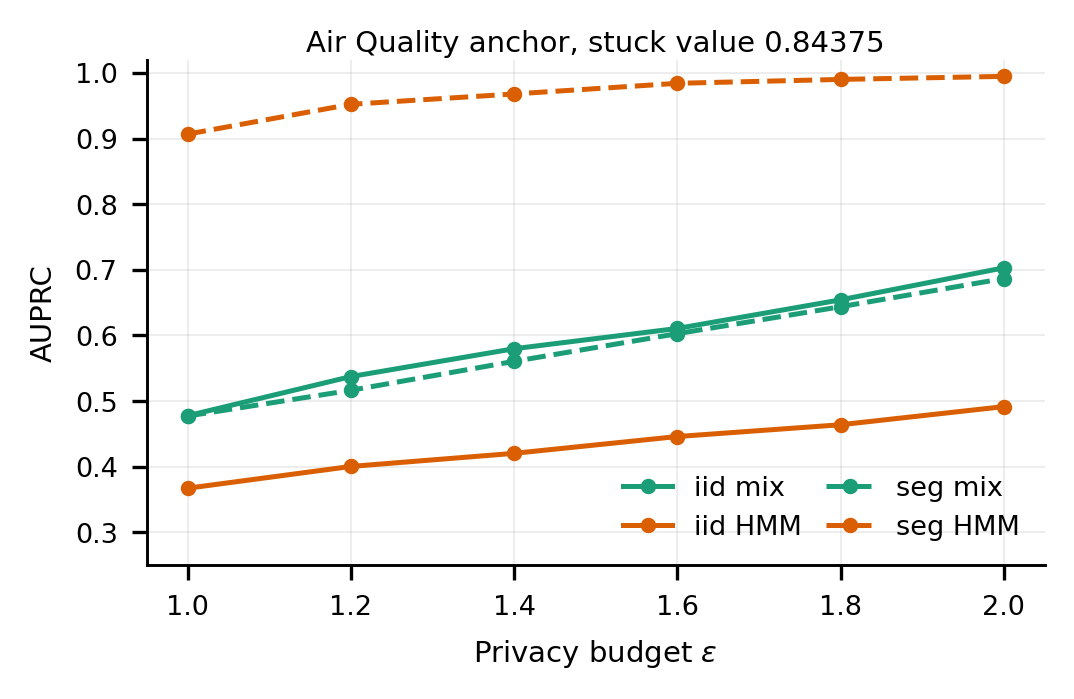
\includegraphics[width=\columnwidth]{results/fig_main_air_quality_compact.png}
\caption{Air Quality anchor AUPRC at stuck value \(0.84375\). Detection improves with privacy budget and model match: the HMM is favorable for persistent segment faults, while the iid mixture is stronger for iid faults.}
\label{fig:air_quality_anchor}
\end{figure}

Fig.~\ref{fig:air_quality_anchor} shows the same model-match pattern used in the broader evaluation. For persistent segment faults at \(a=0.84375\), PrivSAF-HMM improves from \(0.957/0.907\) AUROC/AUPRC at \(\varepsilon=1.0\) to \(0.998/0.995\) at \(\varepsilon=2.0\). For iid injected faults, the temporal persistence assumption is mismatched, and the independent mixture model is stronger: at \(\varepsilon=2.0\), the mixture model reaches \(0.859/0.703\), whereas HMM reaches \(0.712/0.492\). The artifact also records ratio and stuck-bucket diagnostics, because PrivSAF emits repair and audit quantities rather than only anomaly scores.

\subsection{Channel and Model-Match Results}
\label{ssec:q1_channel}

The channel-advantage diagnostic isolates the paper's main modeling claim: after PM-LDP, a raw stuck-at segment is better described as a known PM emission distribution than as a repeated privatized value. Each setting compares bucket-count evidence with a known-channel likelihood-ratio score under the same PM mechanism. Across 420 settings, \(53.6\%\) of the \(\varepsilon=0.5\) settings have bucket AUROC at most \(0.55\) while the known-channel LLR reaches at least \(0.70\). The median gap remains large at \(\varepsilon=1.0\), where bucket AUROC is \(0.566\) and LLR AUROC is \(0.942\).

\begin{figure}[t]
\centering
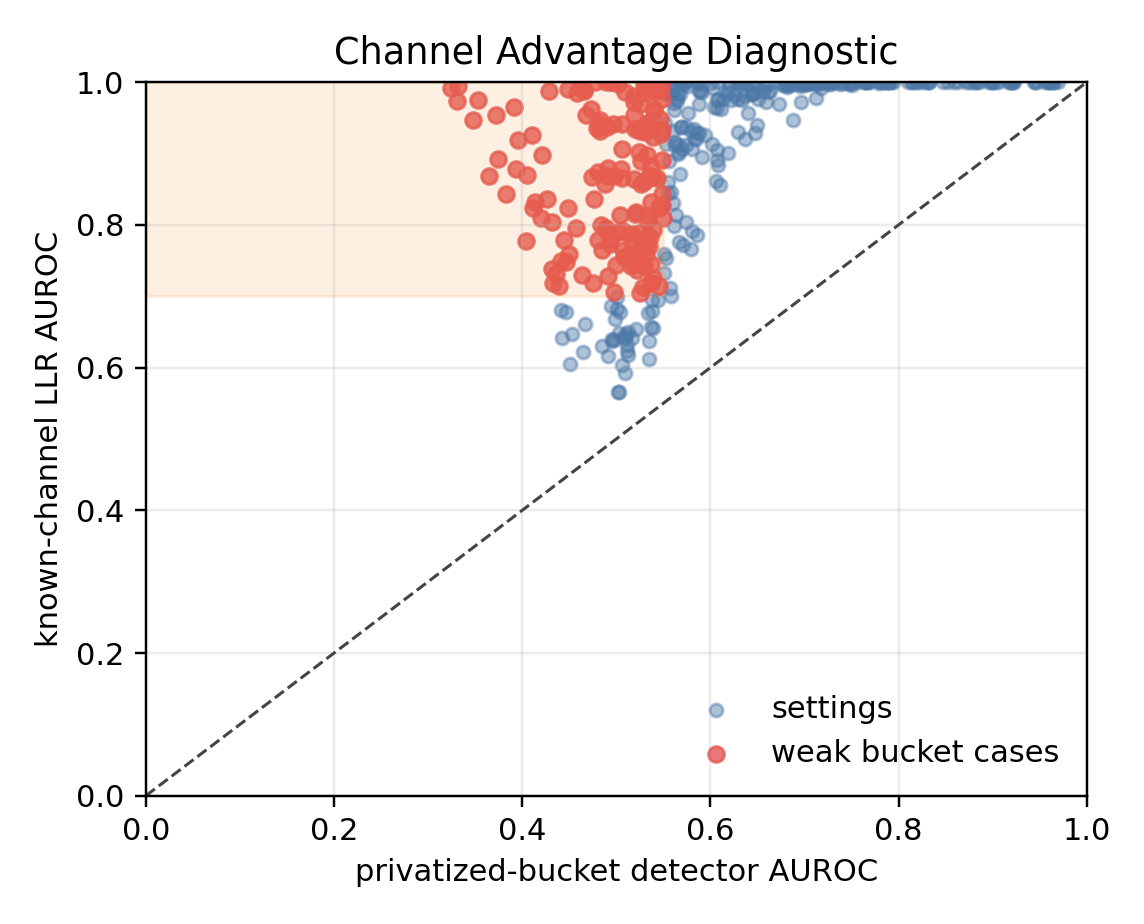
\includegraphics[width=\columnwidth]{fig_icde_channel_advantage.png}
\caption{Channel-advantage diagnostic comparing repeated privatized buckets with declared-channel likelihood ratios.}
\label{fig:icde_channel_advantage}
\end{figure}

This diagnostic shows that private stuck-at cleaning should use the declared channel matrix when available; repeated privatized values are not a reliable surrogate for raw flatlines.

\noindent\emph{Five-stream model-match grid.}
\label{ssec:icde_revision_grid}

The multi-dataset experiment runs Air Quality, Household Power, Bike Sharing, Beijing Air, and NAB machine temperature with iid, segment, and template stuck-at faults. For \(\varepsilon\in\{2,4\}\) and three seeds, 19 scoring methods produce 3,420 detection rows; same-protocol extensions add 1,050 PM-adapted anomaly rows and 750 direct channel-aware rows. Nine posterior-mask repair-aid configurations produce 1,620 repair rows. Fig.~\ref{fig:icde_detection_summary} averages over five datasets, two budgets, and three seeds.

\begin{figure}[t]
\centering
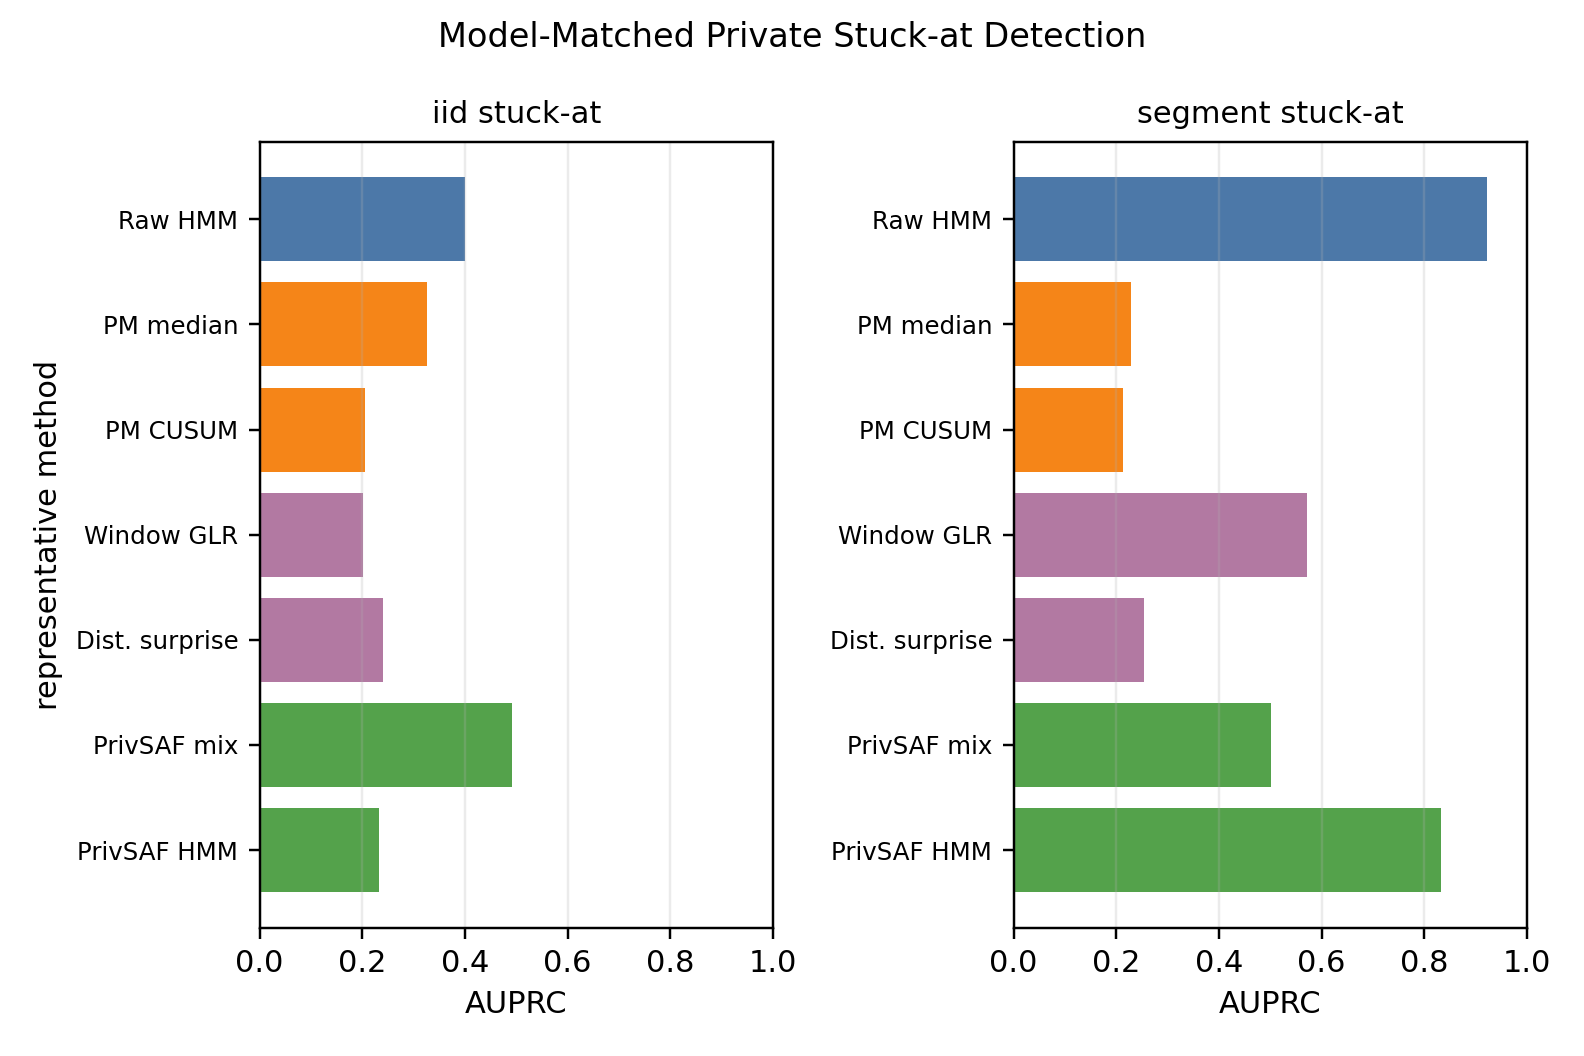
\includegraphics[width=\columnwidth]{results/fig_icde_revision_baselines.png}
\caption{Model-matched detection summary across five streams, two privacy budgets, and three seeds.}
\label{fig:icde_detection_summary}
\end{figure}

Fig.~\ref{fig:icde_detection_summary} shows the model-match pattern. PrivSAF mixture is strongest for iid stuck-at points at \(0.761/0.493\) AUROC/AUPRC, versus \(0.600/0.280\) for the best PM-adapted anomaly baseline. PrivSAF-HMM is strongest for segment faults at \(0.930/0.833\), close to Raw-HMM \(0.948/0.923\) and above the best PM-adapted anomaly baseline \(0.765/0.458\). Generic PM-HMM is the strongest non-PrivSAF channel-aware temporal control for persistent/template faults, but remains below the stuck-column HMM.

\begin{figure}[t]
\centering
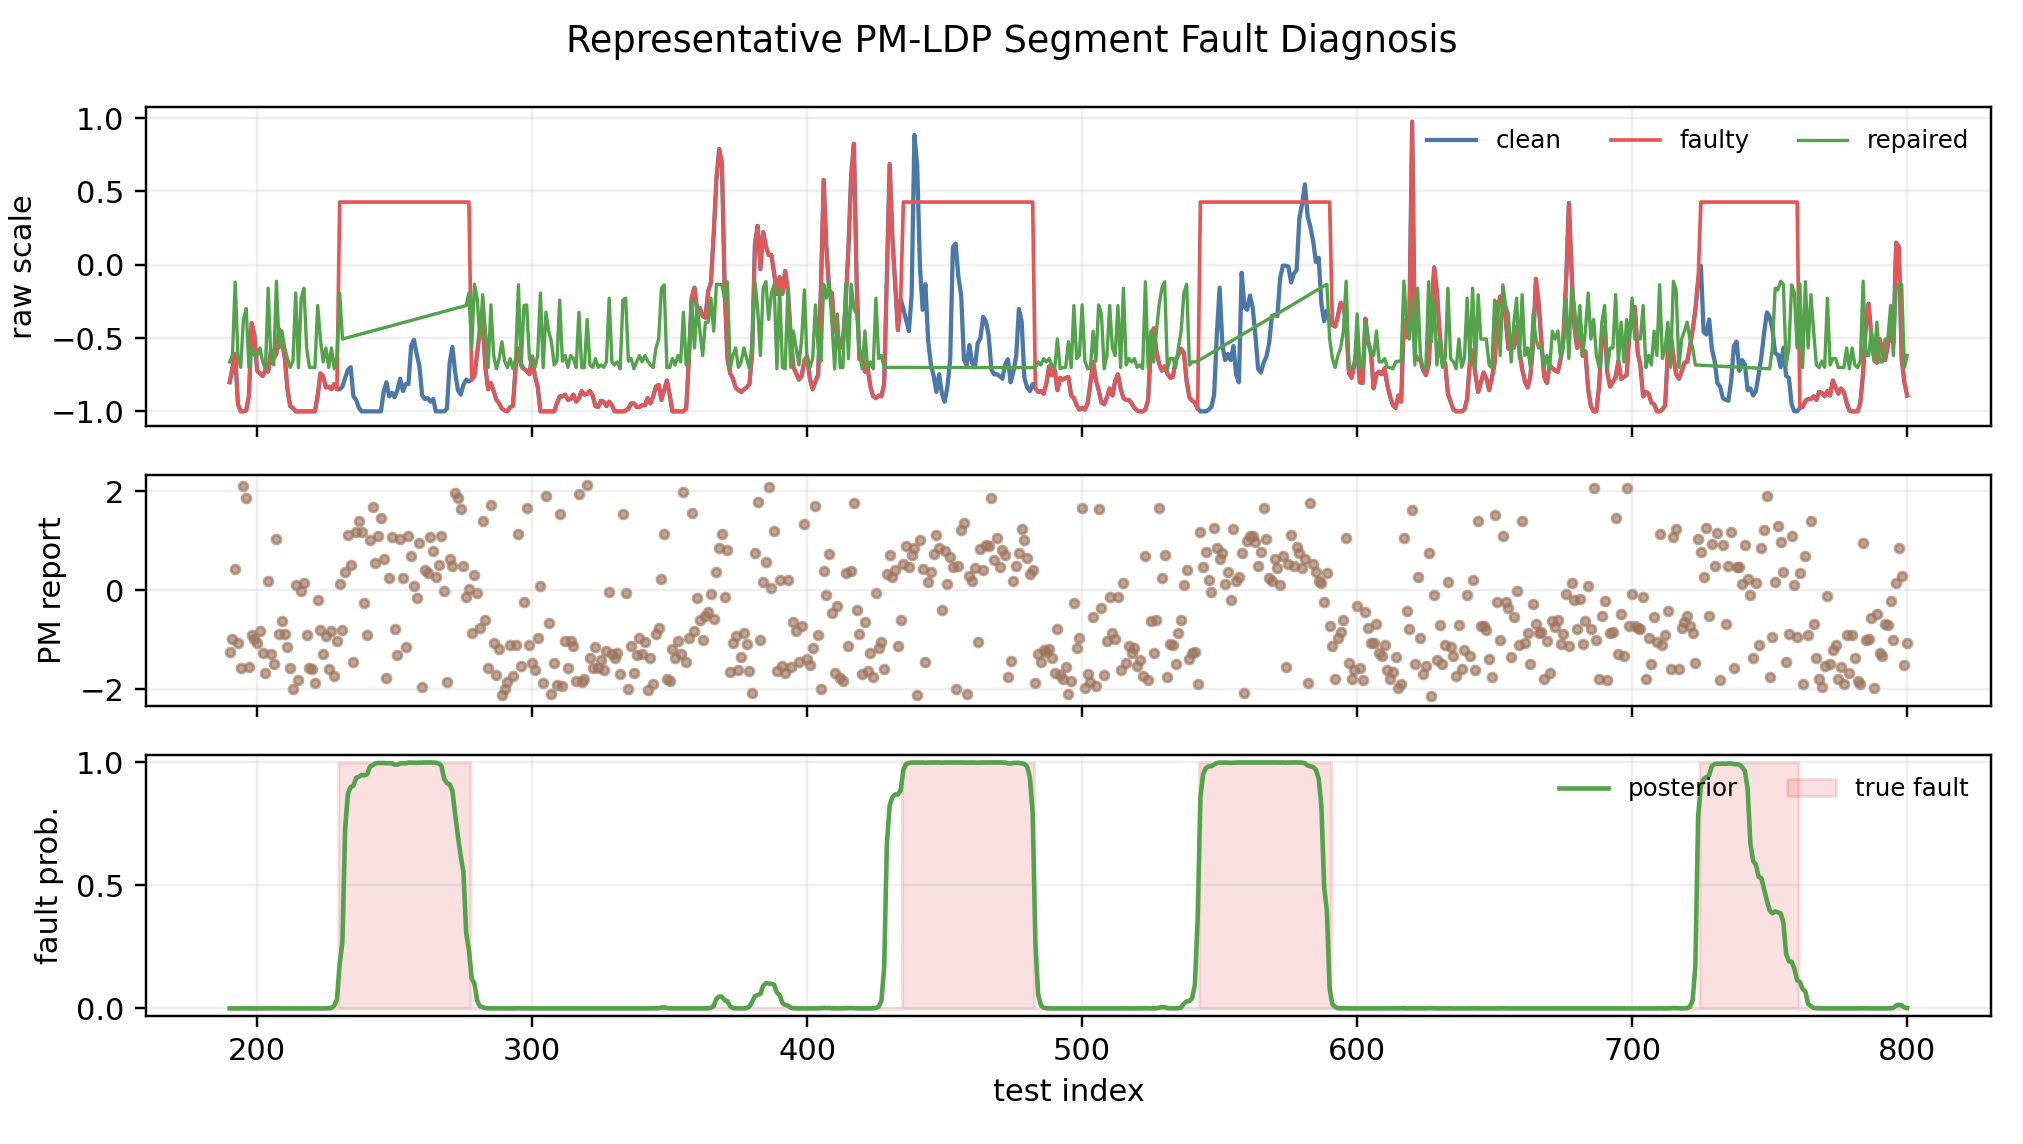
\includegraphics[width=\columnwidth]{fig_icde_representative_timeline.png}
\caption{Representative private stuck-at timeline. The server sees randomized PM reports, not raw flatlines, and the posterior stream tracks the injected stuck-at interval through the declared-channel HMM.}
\label{fig:representative_timeline}
\end{figure}

The representative timeline in Fig.~\ref{fig:representative_timeline} illustrates the deployment setting behind the aggregate scores. The raw stuck segment is visible to the simulator but not to the server; after PM-LDP, the report stream is noisy and does not form an ordinary repeated-value run. PrivSAF recovers the interval through the known channel and temporal posterior, which is why the model is evaluated as a channel-aware post-processing operator rather than as a raw flatline detector.

The model-matched success tier also includes repeated-value and availability semantics, summarized in Table~\ref{tab:router_map}. The HadISD RSS straight-string panel reaches \(0.969/0.896\) AUROC/AUPRC, and the injected dropout-availability panel reaches \(0.992/0.970\). These rows support the same claim as the tail segment grid: PrivSAF is strongest when the label semantics match scalar repeated-value, stuck-column, or explicit-availability emissions. Boundary cases are analyzed separately in Sec.~\ref{ssec:separation_diagnostic} rather than counted as model-matched PrivSAF successes.

Channel miscalibration directly hurts the temporal model, as summarized in Fig.~\ref{fig:icde_channel_ablation}. The calibrated HMM uses the declared PM channel, while wrong-channel variants replace the emission matrix with \(\varepsilon/2\) or \(2\varepsilon\). For segment stuck-at faults, the correctly calibrated PrivSAF-HMM reaches \(0.930/0.833\), while using \(2\varepsilon\) in the HMM emission matrix drops performance to \(0.671/0.505\). On template faults, the correct channel reaches \(0.851/0.613\), compared with \(0.791/0.547\) for \(\varepsilon/2\) and \(0.770/0.545\) for \(2\varepsilon\). These ablations support the main claim that the known LDP channel is useful calibration information rather than incidental noise.

PrivSAF also emits diagnostic quantities rather than only anomaly scores. Averaged over five datasets, two privacy budgets, and three seeds, the iid mixture has ratio MAE \(0.081\), bucket top-1 \(0.700\), and Brier \(0.139\); the segment HMM has ratio MAE \(0.055\), bucket top-1 \(0.800\), and Brier \(0.093\); the template HMM has ratio MAE \(0.087\), bucket top-1 \(0.800\), and Brier \(0.164\). These outputs are absent from PM-adapted anomaly operators, likelihood scans, CUSUM, and window GLR; a generic PM-HMM can fit a free fault emission but does not impose the stuck-column structure used for bucket and posterior-mask diagnostics.

\begin{figure}[t]
\centering
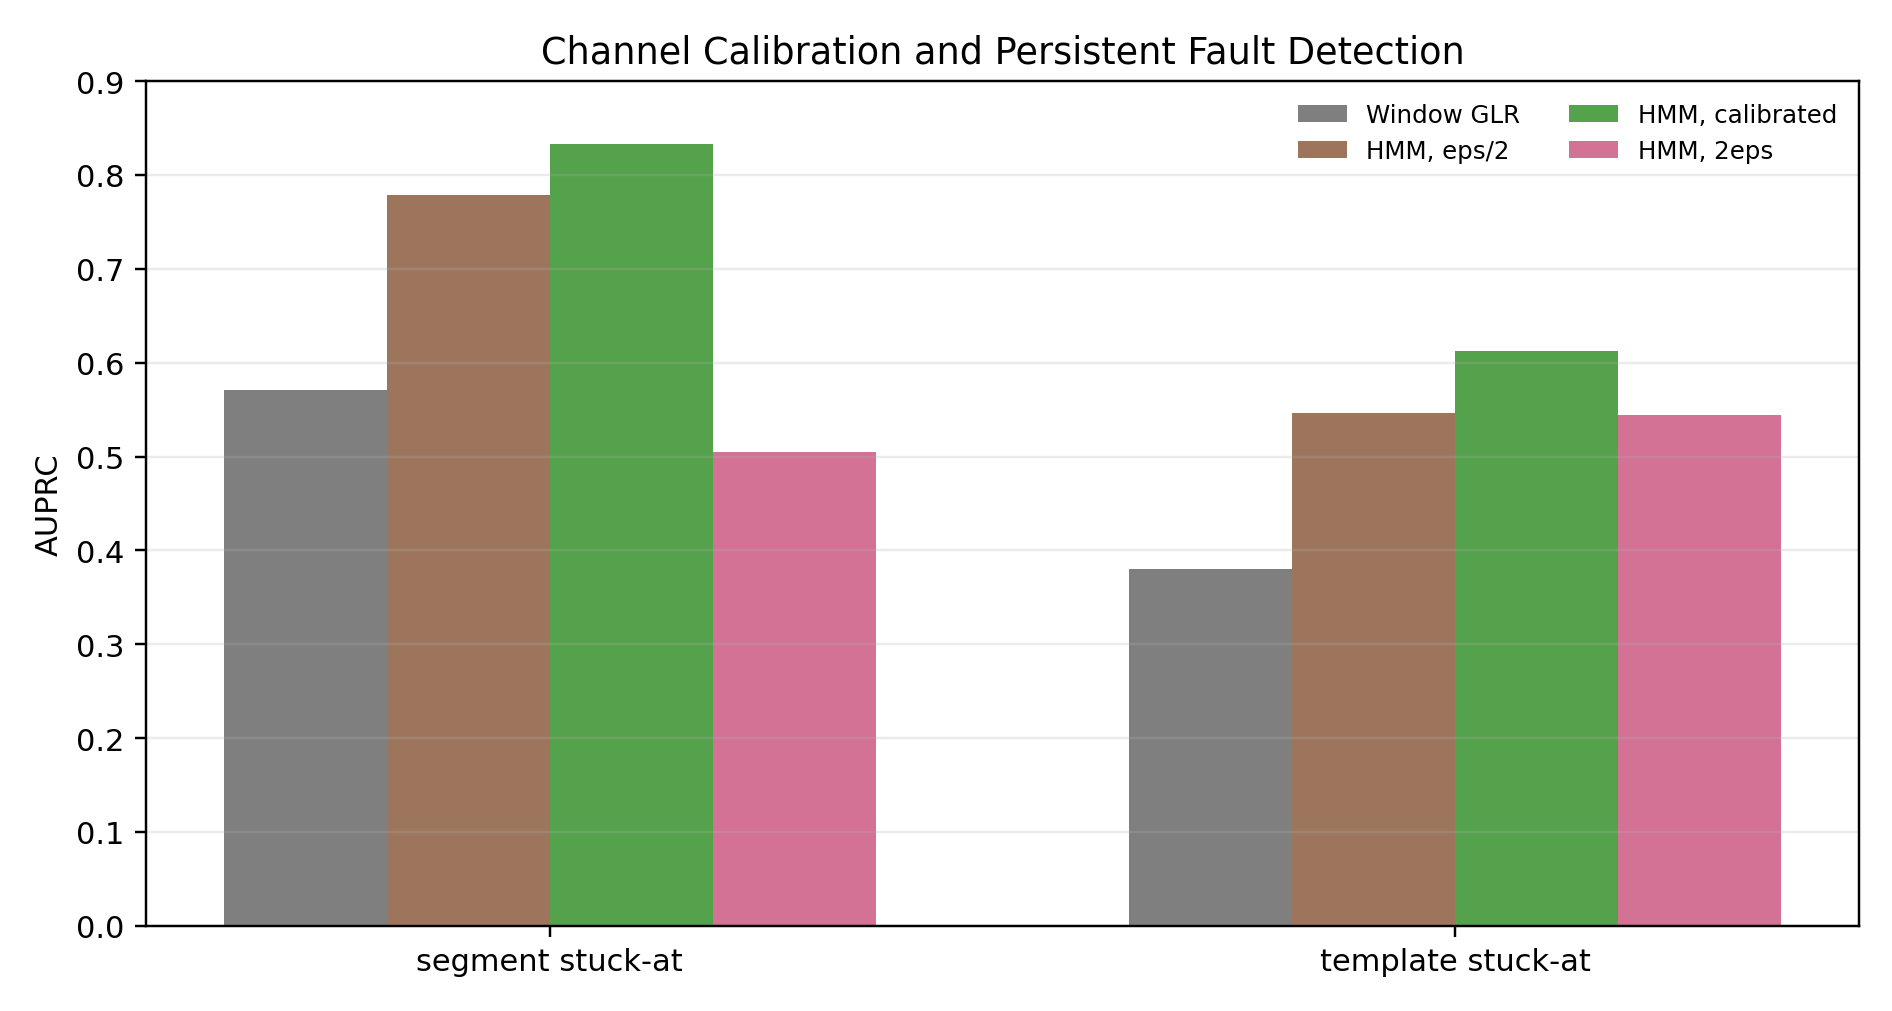
\includegraphics[width=\columnwidth]{fig_icde_channel_ablation.png}
\caption{Calibrated versus wrong-channel HMM emissions for segment and template faults.}
\label{fig:icde_channel_ablation}
\end{figure}

\subsection{Boundary, Real Labels, and Repair}
\label{ssec:separation_diagnostic}

\noindent\emph{Separation audit diagnostic.}
Table~\ref{tab:sep_failure} is the robustness centerpiece. Tail stuck values have larger TV/KL separation and high AUPRC, while median, mode-bucket, and minimum-TV stuck values are often near prevalence even when the channel is correct. Moderate TV/KL separation can still produce weak utility when effective emission overlap remains high. In particular, median \(\varepsilon=2\) and min-TV \(\varepsilon=2\) pass the fixed thresholds but still fail in Table~\ref{tab:sep_failure}; the complete artifact table contains the remaining stress rows.

\begin{table}[t]
\centering
\caption{Separation and failure regimes for PrivSAF-HMM.}
\label{tab:sep_failure}
\scriptsize
\resizebox{\columnwidth}{!}{%
\begin{tabular}{lrrrrr}
\toprule
Stuck value & \(\varepsilon\) & TV & KL & AUPRC & Hit@1 / Prev. \\
\midrule
tail q05 & 2.0 & 0.357 & 0.375 & 0.772 & 0.733 / 0.200 \\
tail q95 & 2.0 & 0.510 & 0.711 & 0.827 & 0.667 / 0.200 \\
median & 0.5 & 0.043 & 0.006 & 0.077 & 0.000 / 0.075 \\
median & 2.0 & 0.229 & 0.136 & 0.085 & 0.067 / 0.075 \\
mode bucket & 1.0 & 0.118 & 0.045 & 0.088 & 0.133 / 0.075 \\
min-TV column & 1.0 & 0.091 & 0.025 & 0.070 & 0.000 / 0.075 \\
min-TV column & 2.0 & 0.225 & 0.130 & 0.079 & 0.050 / 0.075 \\
\bottomrule
\end{tabular}
}
\end{table}

For deployment, Table~\ref{tab:sep_failure} says that central or min-TV stuck values should enter audit/triage even when the channel is correctly specified; tail success cannot be generalized to all scalar buckets.

The separation audit diagnostic passes 40 of 65 controlled tail/central strata and rejects or routes 25. Passing means only that PrivSAF clears the TV/KL diagnostic and enters validation-utility selection. The selected method averages test AUPRC \(0.319\), versus \(0.306\) for ungated PrivSAF; the diagnostic records risk rather than certifying deployment readiness. Table~\ref{tab:false_accept} gives the post-hoc false-accept audit using held-out test labels only for final reporting. With a utility threshold of \(2\times\) prevalence, 22 diagnostic-passing strata are accepted-bad: their mean PrivSAF AUPRC is \(0.0785\) and mean prevalence lift is \(0.903\). These accepted-bad rows show that TV/KL alone cannot certify utility; therefore the policy must abstain unless validation lift clears a threshold.

\begin{table}[t]
\centering
\caption{False accept/reject accounting for the separation audit diagnostic. Mean AUPRC/lift use held-out PrivSAF-HMM utility.}
\label{tab:false_accept}
\scriptsize
\begin{tabular}{lrrr}
\toprule
Bucket & Count & Mean AUPRC & Mean lift \\
\midrule
accepted-good & 18 & 0.903 & 4.51 \\
accepted-bad & 22 & 0.0785 & 0.903 \\
rejected-good & 0 & -- & -- \\
rejected-bad & 25 & 0.0766 & 1.02 \\
\bottomrule
\end{tabular}
\end{table}

For deployment, Table~\ref{tab:false_accept} says that TV/KL is only an admission diagnostic. Final deployment must require validation lift or abstain, because accepted-bad rows show that separation alone does not certify utility.

\noindent\emph{Real-label boundary evidence.}
\label{ssec:acceptability_extensions}

The native flatline and HadISD panels provide the closest boundary evidence for repeated-value semantics. Native flatline windows reach AUPRC \(0.484\) after PM-LDP, close to the identity-channel score \(0.505\). The strongest HadISD case is RSS wind direction, where PrivSAF-HMM reaches \(0.969/0.896\) AUROC/AUPRC; compact replication keeps RSS as the clearest straight-string layer, while low-prevalence nonwind cases remain supporting evidence in the artifact.

NOAA CO-OPS verified six-minute ERDDAP supplies official flat-tolerance labels with values in the same rows~\cite{noaa_coops_verified_erddap,noaa_coops_qc_requirements}. Raw flatness is strong, but the private signal is weak: at \(\varepsilon=2\) and 24 buckets, PrivSAF range-HMM r1 reaches \(0.539/0.0246\) AUROC/AUPRC, above report-frequency and GLR controls but far below a high-accuracy deployment target. Top-\(1\%\) triage gives \(1.57\times\) lift. The router therefore treats CO-OPS as a feasibility row: the official value+label semantics are compatible with range-HMM cleaning, but the measured private lift supports triage/audit rather than automatic repair. This explanation is important because a flat-tolerance label can be semantically compatible while still being statistically weak after LDP randomization.

I-ORS and WSN are boundary cases. I-ORS \(\texttt{SLH\_QC}=5\) behaves like a local QC regime: PM-window GLR reaches AUPRC \(0.716\), above global PrivSAF-HMM \(0.372\), and low-\(\varepsilon\) LLR-CUSUM improves over PrivSAF. WSN prepared row labels similarly favor PM-window GLR \(0.463\) over PrivSAF-HMM \(0.296\). The boundary ledger records these as semantic mismatches rather than hiding them as PrivSAF failures.

The streaming panel evaluates the online top-\(k\) implementation on segment stuck-at faults. Full candidate enumeration remains more accurate at \(0.930/0.833\), while the top-8 online HMM obtains \(0.813/0.594\) and reduces average per-frame runtime from \(0.374\) ms to \(0.125\) ms. This establishes the implementation tradeoff used for longer streams: full search is preferred when latency permits, and the streaming shortlist gives a fixed-memory approximation when low per-frame cost is required.

Posterior-mask repair is evaluated as a downstream analytics operator rather than as ground-truth reconstruction. In the repair grid over five streams, iid/segment faults, and three seeds, no repair has MAE \(0.1758\), fault-point MAE \(0.8789\), clean-point damage \(0\), downstream mean error \(0.1664\), and exceedance-count error \(174.0\). PrivSAF top-\(k\) mask repair reduces these to \(0.1470\), \(0.5840\), \(0.0377\), \(0.1136\), and \(112.9\). Oracle-mask interpolation remains much stronger with MAE \(0.0463\), so the repair result supports the database view interface and conservative aggregate improvement; raw-value reconstruction remains outside the claim.

\begin{figure}[t]
\centering
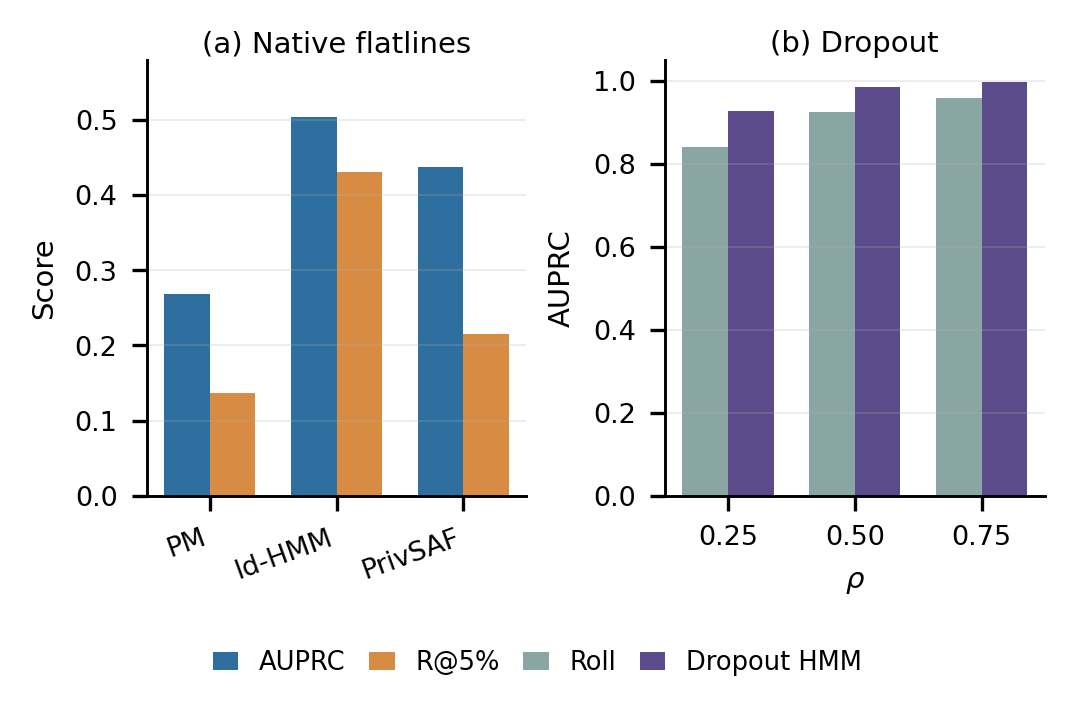
\includegraphics[width=\columnwidth]{results/fig_main_boundary_compact.png}
\caption{Compact boundary evidence. Native weak-label flatlines are useful but conservative after PM-LDP; explicit availability uses a compatible dropout HMM and remains a high-AUPRC setting.}
\label{fig:boundary_repair_panels}
\end{figure}

Fig.~\ref{fig:boundary_repair_panels} keeps the two visual boundary cases that fit a single column: native repeated-value evidence is useful but conservative after PM-LDP, while explicit availability is a distinct emission model with high utility. Sensitivity and repair results are retained in the surrounding text and in the repair-aware SQL workload, where posterior masks improve downstream aggregates without claiming oracle-level raw reconstruction.

\noindent\emph{Sensitivity and mechanism checks.}
\label{ssec:stress_diagnostics}

A compact mechanism extension tests the channel-matrix interface beyond PM. Replacing PM with the Duchi binary real-valued LDP mechanism keeps the same inference code: only \(M\) and the report alphabet change. On Air Quality segment stuck-at faults, the Duchi-binary HMM reaches AUPRC \(0.737\) at \(\varepsilon=1\) and \(0.939\) at \(\varepsilon=2\); at \(\varepsilon=0.5\), window GLR is selected (\(0.481\) versus \(0.220\)). The extension verifies that the stuck-at posterior code is tied to a declared scalar channel matrix rather than PM-specific likelihoods.

Additional failure-mode checks are recorded in the artifact. Calibration contamination is stable up to \(10\%\) stuck-bucket contamination and drops sharply at \(20\%\) or higher. Bucket counts from \(8\) to \(64\) give similar AUPRC while runtime grows with the number of candidates. The \(\varepsilon\)-mismatch curve is strongest near the declared budget and weakens when inference assumes a much larger budget. Short multi-device traces remain usable but are noisier: at length \(64\), AUPRC ranges from \(0.647\) to \(0.852\), while length \(256\) reaches \(0.865\), \(0.921\), and \(0.926\) for \(4\), \(16\), and \(32\) devices.

The same experiments also record diagnostics for the separation assumptions used in the theory. Averaged over datasets and stuck values, the normal--fault PM emission \(L_1\) separation increases from \(0.867\) at \(\varepsilon=2\) to \(1.423\) at \(\varepsilon=4\), and the minimum adjacent-column total variation increases from \(0.054\) to \(0.200\). These empirical diagnostics match Proposition~\ref{prop:pm-separation}: higher per-report privacy budget yields better-separated PM emissions, which is exactly the regime where the HMM and mixture estimators improve.

The stress grid confirms the harder central-value regime. On median, mode-bucket, and minimum-TV stuck columns, matched-calibration PrivSAF-HMM averages only AUPRC \(0.0806\), \(0.0766\), and \(0.0906\) at \(\varepsilon=0.5,1,2\), close to the mean fault prevalence \(0.075\). Bucket hit@1 is \(0.0167\), \(0.0444\), and \(0.1111\). For the hardest minimum-TV column, HMM AUPRC is \(0.0813\), \(0.0698\), and \(0.0788\), with TV separation \(0.0406\), \(0.0908\), and \(0.2250\). The validation-shifted calibration rows are also reported; in this split they increase mean HMM AUPRC to \(0.1364\), so the paper treats calibration shift as an audited sensitivity condition rather than assuming it always hurts. Across 1,080 HMM rows, AUPRC correlates positively with TV separation (\(0.353\)) and KL separation (\(0.411\)), which is consistent with the separation propositions and exposes the low-separation failure regime.

\subsection{Auditability and Repair-Aware Queries}
\label{ssec:q5_db}

The deployment interface is a channel-aware stuck-at/flatline policy over the private scalar telemetry ledger. It consumes mechanism, budget, report alphabet, calibration row, optional availability symbol, label semantics, TV/KL diagnostics, validation-lift threshold, and cost weight, then stores the selected operator state as invocation metadata and provenance. The cleaning plan binds semantics to eligible methods: persistent scalar stuck-at segments, HadISD straight strings, and CO-OPS flat-tolerance labels use PrivSAF-HMM or range-HMM when validated; iid point stuck-at uses the mixture posterior; explicit availability uses the dropout HMM; I-ORS and WSN route to PM-window GLR or LLR-CUSUM as semantic-boundary layers.

The prototype exposes three database-visible interfaces: a batch likelihood view, a keyed posterior stream, and a repair-aware aggregate view. Candidate top-\(k\) lookup drops from \(3822\) ms to \(0.060\) ms with materialized likelihood state; budget checks drop from \(86.3\) ms to \(0.103\) ms and pass the 200k-report verifier; the replay workflow requests \(72{,}000\) microbatch events, accepts \(60{,}000\), rejects \(14{,}000\) by budget, detects \(10{,}000\) duplicates, and propagates 120 corrections; dashboard queries fall from \(91.4\) ms to \(1.34\)--\(1.67\) ms while remaining linked to provenance. The DBMS architecture remains conventional, but the measurements show that the operator contract has concrete physical states and query paths that can be verified across database backends; full environment details remain in the artifact files.

The device-level privacy ledger remains part of the deployment interface. Server-side cleaning choices are post-processing, so they do not consume extra privacy budget; the per-report LDP cost is still determined by the client-side mechanism. Long-running deployments should combine PrivSAF with report caps, contribution limits, or a longitudinal privacy accountant.

Validation labels and router evidence are public benchmark evidence in this paper. In a real deployment, sensitive validation labels require separate accounting or access control, and label-sparse deployments should use the operator in audit/triage mode until validation lift can be estimated. This validation dependency is a deployment requirement rather than a tuning convenience: Table~\ref{tab:false_accept} shows that separation alone can admit low-utility strata, so each routed layer should store validation source, lift threshold, and abstention reason in the policy ledger.

\begin{table}[t]
\centering
\caption{Expanded repair-aware SQL workload.}
\label{tab:sql_workload}
\scriptsize
\setlength{\tabcolsep}{2pt}
\renewcommand{\arraystretch}{0.9}
\begin{tabularx}{\columnwidth}{p{0.31\linewidth}Y}
\toprule
Query & SQL intent and evaluation result \\
\midrule
Hourly mean & Group by posterior mask; mean error \(0.1664\rightarrow0.1136\). \\
Exceedance count & Count repaired threshold values; error \(174.0\rightarrow112.9\). \\
Suspicious top-\(k\) & Rank materialized posterior state; lookup \(3822\) ms \(\rightarrow0.060\) ms. \\
Budget audit & Join privacy ledger and budget trace; check \(86.3\) ms \(\rightarrow0.103\) ms. \\
Provenance drilldown & Trace report, channel, calibration, and policy versions; 200k-report verifier passes. \\
\bottomrule
\end{tabularx}
\end{table}

\section{Related Work}
\label{sec:related}

LDP telemetry protects each report before collection and supports frequency,
telemetry, and real-valued analytics
\cite{kasiviswanathan2011what,dworkroth2014,duchi2013localprivacy,
erlingsson2014rappor,nguyen2016harmony,ding2017telemetry,
wang2019multidimensional}. These mechanisms are usually used to estimate
population statistics, histograms, heavy hitters, or means from privatized
reports. PrivSAF is complementary: it does not introduce a new local
randomizer or estimator. Instead, it treats the declared scalar LDP mechanism
as an observation channel for server-side cleaning after collection. This
distinction is important because a pre-randomization stuck-at fault is not an
ordinary noisy outlier in the stored table; after local randomization, the
server observes only channel outputs whose likelihood depends on the declared
mechanism and calibration.

EM and HMM inference are standard tools for incomplete-data and temporal
latent-state models \cite{dempster1977em,rabiner1989hmm}. PrivSAF does not
claim novelty in these routines. Its distinction is the channel-constrained
emissions \(M\boldsymbol{\alpha}\) and \(M_{:,s}\): the normal state marginalizes
the calibrated raw distribution through the declared channel, whereas a stuck
state corresponds to a specific channel column. Thus the latent explanation is
not merely a free report-space cluster or anomaly state; it remains tied to a
raw bucket under the LDP mechanism. In addition, posterior scores are not used
as transient classifier outputs. They are materialized as versioned database
records with channel, calibration, policy, privacy-ledger, and replay lineage.

Sensor fault diagnosis and time-series anomaly detection cover many
non-private faults and anomaly families
\cite{isermann2005fault,chen2006distributedfault,chen2013faultresilient,
chandola2009anomaly,lavin2015nab,ahmad2017nab,xu2021anomaly,
deng2021graph,li2021multivariate,audibert2020usad}. These methods typically
assume that the monitoring system observes the signal, residuals, or feature
vectors on which faults are expressed. PrivSAF addresses a narrower but
different setting: scalar stuck-at/flatline faults occur before privatization,
while the server observes only private reports. Consequently, repeated raw
values do not appear as repeated stored values, and standard flatline rules are
not directly applicable. The experiments therefore compare against
PM-adapted anomaly baselines, channel-aware scans, LLR-CUSUM, and generic
PM-HMM under the same private telemetry ledger. The goal is not to dominate
general anomaly detection, but to decide when a stuck-at interpretation is
semantically compatible with the declared LDP channel and when the system
should route or abstain.

Database provenance, cleaning, private data systems, and audit-oriented data
management provide the closest systems context
\cite{cui2000lineage,buneman2001whywhere}. Prior data-management work provides
lineage for derived tuples, repair frameworks for observed dirty data, and
policy mechanisms for protected computation. PrivSAF uses these ideas in a
different contract. Its input relation already consists of privatized reports;
the operator is therefore a post-processing step rather than a new collection
mechanism. The database state must record not only which reports contributed
to a posterior decision, but also which declared channel, calibration snapshot,
policy thresholds, validation evidence, and privacy-ledger entries made that
decision admissible. Replay is correspondingly triggered by changes in
mechanism metadata, calibration, policy, or validation evidence, not only by
changes in base reports.

PrivSAF also differs from data-cleaning systems that repair observed dirty
values. Here the raw value that became stuck is never observed by the server,
and the repeated-value symptom is destroyed by local randomization. The
resulting action must therefore be a posterior record tied to a declared LDP
channel and replayable metadata, not a direct overwrite of a dirty cell.


\section{Conclusion}
\label{sec:conclusion}

PrivSAF is an auditable known-channel database operator for scalar LDP stuck-at/flatline telemetry. It ties the \(M\alpha\)/\(M_{:,s}\) kernel to mechanism metadata, calibration, routing policy, posterior state, privacy/provenance accounting, replay/correction lineage, and repair-aware SQL aggregates. Controlled faults show model-matched successes and diagnostic-passing failures; native, HadISD, CO-OPS, I-ORS, and WSN rows define the deployment boundary. The operator should be used when semantics, separation, and validation lift support stuck-column inference.

\section*{Acknowledgment}

AI tools were used for language editing and script-drafting assistance. The authors reviewed all generated content, and all numerical results were produced by project scripts and checked against recorded outputs.

\bibliographystyle{IEEEtran}
\bibliography{references}

\end{document}
